
\documentclass[12pt,a4paper]{article}

\usepackage{pdflscape}
\setlength{\textwidth}{165mm}
\setlength{\textheight}{235mm}
\setlength{\oddsidemargin}{-0mm}
\setlength{\topmargin}{-10mm}

\usepackage{mathtools}
\DeclarePairedDelimiter\abs{\lvert}{\rvert}%
\DeclarePairedDelimiter\norm{\lVert}{\rVert}%
% Swap the definition of \abs* and \norm*, so that \abs
% and \norm resizes the size of the brackets, and the
% starred version does not.
\makeatletter
\let\oldabs\abs
\def\abs{\@ifstar{\oldabs}{\oldabs*}}
%
\let\oldnorm\norm
\def\norm{\@ifstar{\oldnorm}{\oldnorm*}}
\makeatother

\newcommand*{\Value}{\frac{1}{2}x^2}%
%\usepackage{graphicx}
\usepackage{graphicx}
\usepackage{subfigure}%exclusive to subcaption
%\usepackage{subcaption, float} 
\usepackage{xcolor}
\definecolor{ggray}{RGB}{47,79,79}
\definecolor{firebrick}{RGB}{178,34,34}
\definecolor{green1}{RGB}{50,205,50}
\definecolor{umbrella}{RGB}{0,191,255}

\usepackage{pgfplots}
\usepackage{tikz}
\usetikzlibrary{patterns,arrows,shapes,positioning,shadows,trees}
\tikzstyle{every node}=[draw=black,thick,anchor=west]
\tikzstyle{selected}=[draw=red,fill=red!30]
\tikzstyle{optional}=[dashed,fill=gray!50]
\tikzstyle{neglected}=[dashed]

\usepackage{amsfonts}
\usepackage{amssymb,amsmath} %  $\displaystyle \sum$ will print a bigger one Σ , like in equations  in amsmath package

\DeclareMathOperator{\sgn}{sgn}

\usepackage{soul}

\usepackage{titlesec}
\titleformat*{\section}{\Large\sffamily}
\titleformat*{\subsection}{\large\sffamily}
\titleformat*{\subsubsection}{\itshape \sffamily}


%\renewcommand{\refname}{參考文獻}
\usepackage[nottoc]{tocbibind}
%\settocbibname{參考文獻}
\usepackage{float}
\usepackage{multirow}
\usepackage{booktabs}
%\usepackage[square]{natbib}

\title{Numerical Analysis HW09 : Polynomial Interpolations}
\author{Ming-Chang Chiu 100060007}
\date{\today}
\begin{document}
\maketitle
\fontsize{12}{20pt}\selectfont %本行指令第一個12是字體大小、第二個20是行距,selectfont一定要加才會發生效果。但此指令只對正文有效,註解無效

\section{Objective}
In this assignment, we are given different numbers of support points in each .dat file, with $475 \le x \le 775$. We are required to use Lagrange interpolation to interpolate the Y values for each $475 \le x \le 775$ and then observe the results as well as the difference between given values and interpolated values. I implemented\\ 

double Lagrange(double x,VEC $\&$XDATA,VEC $\&$YDATA);\\\\
as my interpolating function.

\section{Implementation of Lagrange}
In my implementation, I use the non-recursive form of Neville's algorithm.The theorem of Neville's algorithm is like the following:\\ Given n+1 support points ($x_i,y_i$), $i=0...n$, with $x_j \neq x_k$ if $j \neq k$, then the Lagrange interpolation at the point $x$, $F_{0 \dotsc n}\left( x \right)$, can be calculated using the following recursion formula:\\	
$$F_{i}\left( x \right) = y_i$$
$$F_{{i_0}{i_1}\dotsc{i_k}}(x) = \frac{ (x-x_0)F_{{i_1}{i_2}\dotsc{i_k}}(x)  -  (x-x_{i_k})F_{{i_0}{i_1}\dotsc{i_{k-1}}}(x) }{ x_{i_k} - x_{i_0} }$$
I implemented its non-recursive form for efficiency issue. I create an array, NS, to store the intermediate value such as $F_{23}$ etc.; in each iteration of $for loop$, part of the NS will be updated and then given to next iteration. Finally the interpolated result will be stored in NS[0] and returned. The whole code snippet can be viewed as follow:
\begin{figure}[H]
  \centering
      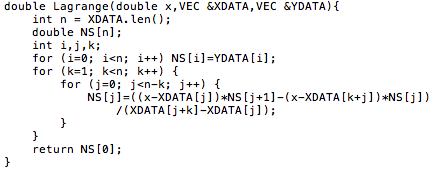
\includegraphics[width=1\textwidth]{./lagr.jpg}
 % \caption{Interpolation with 13 given pairs of (X,Y)}
\end{figure}

\section{Workflow}

\begin{description}  

\item [Usage:] For example,  ./hw09.out $<$ f3.dat
\item [Solve:] Non-recursive Neville's algorithm is applied.
\item[Desired output:] The program will build a file named $data.txt$, which will store value of $x_i$, interpolated value, error at $x_i$, and original value at $x_i$ in f301.dat sequentially each row. One can load the .txt file for further analysis.
\end{description}

\section{Results}
  \begin{center}
    \begin{tabular}{|c|c|c|}
    \hline  Input File & Max error & Max error within $550 \le x \le 700$  \\
    \hline  f3.dat	&372.8669    	&372.8669	\\
    \hline  f5.dat	&248.3406    	&233.3644	\\
    \hline  f7.dat	&379.1073    	&147.5782	\\
    \hline  f13.dat	&1283.4489 	&39.6189	\\
    \hline  f21.dat	&16728.5648	& 17.804	\\\hline
 \end{tabular}

 \end{center}


\section{Plot Analysis}
The error is defined as $| Lagrange(x_i) - f301(x_i) |$
\begin{figure}[h!]
  \centering
      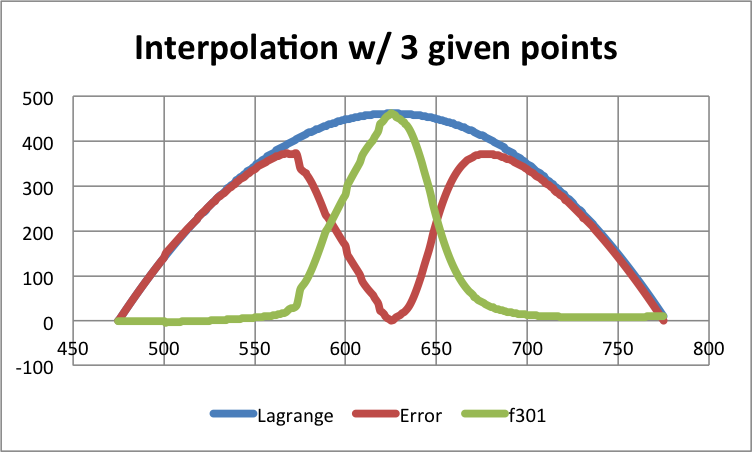
\includegraphics[width=1\textwidth]{./3.png}
  \caption{Interpolation with 3 support points}
\end{figure}
\newpage
\begin{figure}[h!]
  \centering
      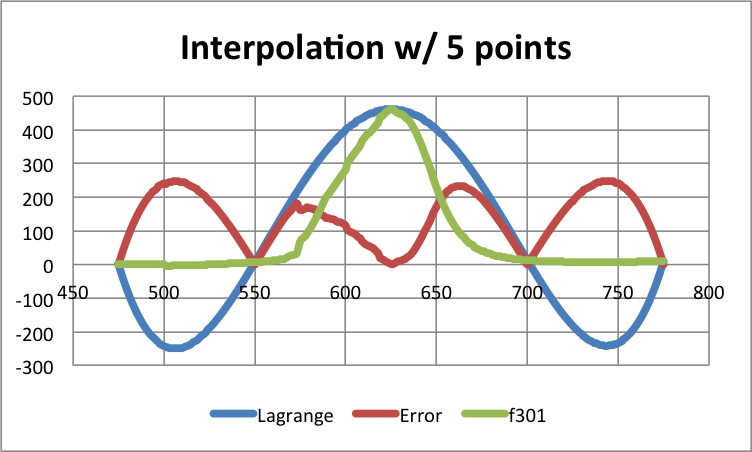
\includegraphics[width=1\textwidth]{./5.png}
  \caption{Interpolation with 5 support points}
\end{figure}
\begin{figure}[h!]
  \centering
      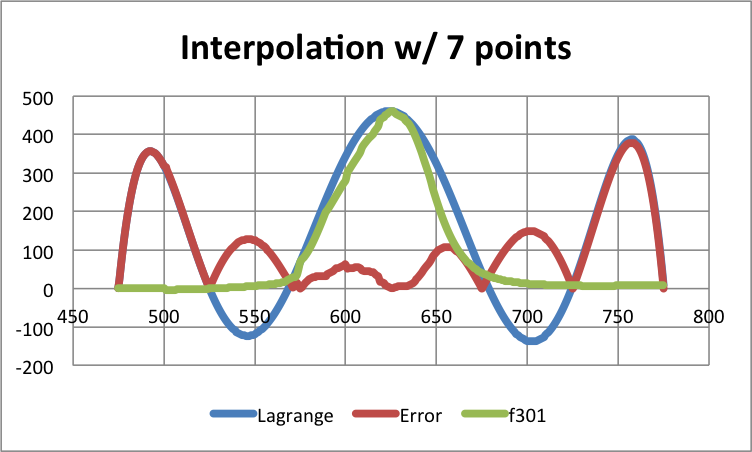
\includegraphics[width=1\textwidth]{./7.png}
  \caption{Interpolation with 7 support points}
\end{figure}
\begin{figure}[h!]
  \centering
      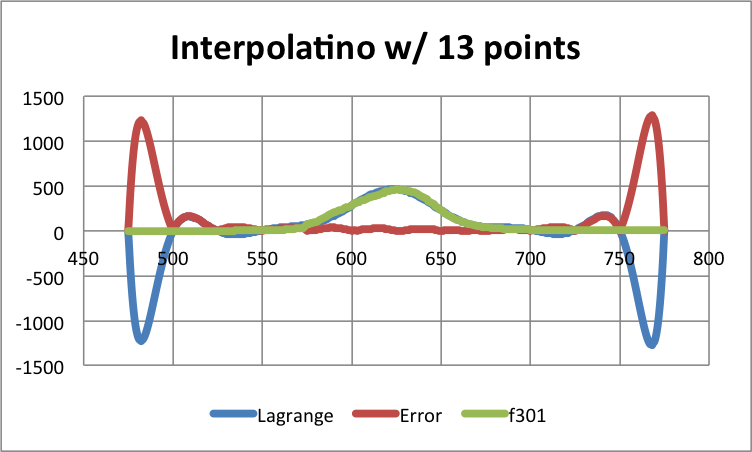
\includegraphics[width=1\textwidth]{./13.png}
  \caption{Interpolation with 13 support points}
\end{figure}
\begin{figure}[h!]
  \centering
      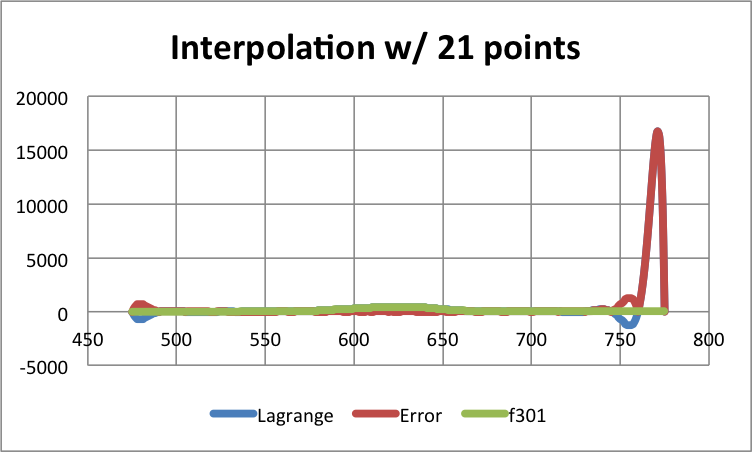
\includegraphics[width=1\textwidth]{./21.png}
  \caption{Interpolation with 21 support points}
\end{figure}


\section{Observations}
In general, I would expect that with more support points, the more approximate the interpolated waveform will be. The result tells me that it is partially true.
From Figure1, we can see that at the center of interval [475,775] the error is the smallest and it will ascend and then descend as $X$ increases or decreases, the error plot is like a humped camel's back. This is because we have only three support points and the order of Lagrange interpolation is 2.

In sum, from the table in Section 4, the maximal error within [550,700] is decreasing as the order of Lagrange formula increases(i.e. more support points), which means Lagrange is more and more approximate to the original waveform. But for all range of $X$, the output could have very large numerical error. From my plots, at right and left side of these plots, the error is getting larger since f5.dat, a extreme case is: in Figure 5, with 21 support points, Lagrange formula order is 20, the error can reach about 16728, which is quite massive. But the waveforms of Lagrange and f301 overall tend to be more and more similar within [550,700] as more support points we have, which partially matches my original conjecture.

One interesting thing should be noticed is that in Figure1, 2, 3 and 4, the Lagrange waveforms are symmetric but in Figure 5 the waveform is asymmetric and has extreme numerical error within [750,775](Error and Lagrange behave the same within this interval). 

\end{document} 
